\chapter{Linked Lists}\index{Linked Lists}

\section{Introduction}
\label{ch10-intro}%\hyperlabel{ch10-intro}%

This chapter introduces you to linked lists. In the QDOSMSQ
    operating system, linked lists are used in many places -{} and you can use
    them in your own code as well. This chapter tells you how.

\section{Linked Lists}
\label{ch10-linked-lists}%\hyperlabel{ch10-linked-lists}%

Linked lists are used within QDOSMSQ to hold details of the
    directory devices installed on the system, interrupt routines and so on,
    but what are they exactly?

Imagine that you are writing a program, and you decide that you need
    some storage for some data, let's say a list of people's names and
    addresses. So, how about an array? Well, the problem with that is how many
    entries are you going to allow? If you don't allow enough entries, you
    won't have much of an address book. If you have too many entries then you
    are wasting space. If you sell the program, or give it away, then you need
    to consider the needs of people other than yourself -{} some will need a few
    entries and others, much more. How do you cope?

Well, a linked list could be the answer. You start off with no
    storage defined at all, except for a single, maybe two, variables which
    hold the address in memory of the beginning (and maybe the end) of your
    list of addresses. As you add new contacts to your address book, each one
    is created at some `random' location in memory and linked into your
    existing list of contacts. Hence, you have a linked list.

In a linked list, each entry is called a node, and the pointer to
    the very first entry in the list is known as the root node.

In memory an array, of 10 entries of 100 byte long strings, is
    consecutive. Don't forget the strings have a word at the start defining
    their length, so each entry is actually 102 bytes long. If the first entry
    is located at address 1000 then the next entry is at address 1102, the
    next at 1204 and so on. There are no gaps between entries and you can
    quickly calculate the start address of any particular entry as 
    
    $1000 + (INDEX * 104)$
    
    where INDEX is the entry you are looking for, starting at
    zero.

In a linked list, the nodes are potentially all over the place, the first might
    be at address 1000, the second at 2000, the third at 1200 and so on. There
    is no logical order to the locations and you cannot calculate the address
    of a particular node using any formula as you can with arrays.

What you can do, however, is store away the address of the first
    node in a special node known as the root node, and from that, you can
    navigate along the list from start to finish by finding the address of the
    next node from the data stored in the individual nodes. Our 100 byte long
    strings would be 106 bytes allowing 4 bytes to store the memory address of
    the `next' entry in the list and the obligatory 2 byte length word.
    However, think about that 102 bytes in each entry of the array -{} you might
    not need all 102 bytes. In our linked list, each node will have 4 bytes
    for the pointer and only as much space as is required by the data, so each
    node need not be $102 + 4$ bytes long. Another saving over the array.

A linked list can be thought of like an old program on UK TV,
    \emph{Treasure Hunt}, where Aneka Rice used to zoom around the country in a
    helicopter picking up clues in one location which told her where to go for
    the next clue and so on, until she found the `treasure' at the end of the
    list of clues. This is exactly what a linked list is.

If we have a node in our list defined as follows, then we can see
    how it looks in memory below. Each node in the list will look like Figure~\ref{fig:LinkedListNodeStructure} with a 4 byte pointer at the start holding the address of the next node in the list, and everything from byte 4 onwards holding some form of desired data.

\begin{figure}[h]
\center
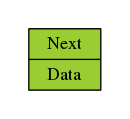
\includegraphics[width=0.2\textwidth]{Content/images/LL_Single_node.png}
\caption{Linked List Node Structure.}
\label{fig:LinkedListNodeStructure}
\end{figure}

The root node, as mentioned above, is special. It has no data part,
    only the pointer part, although it is not necessary for it not to be a full node, the data part will be empty in such cases.

The conceptual layout in memory is a bit like Figure~\ref{fig:ASimpleLinkedList} (using the
    addresses mentioned above and assuming the root node lives at address \$ABCD):

\begin{figure}[h]
\center
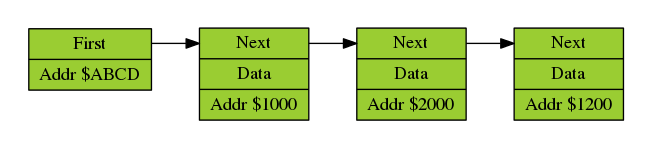
\includegraphics[width=0.95\textwidth]{Content/images/LL_Single_list.png}
\caption{A Simple Linked List.}
\label{fig:ASimpleLinkedList}
\end{figure}

The lowest section of each node above simply shows an example address in memory where that particular node lives. It is not part of the node itself.

In physical terms there are, of course, no handy arrows. Using real values as
    described above in the pointer locations, it would look like Figure~\ref{fig:MemoryOrganisationOfASimpleLinkedList}:

\begin{figure}[h]
\center
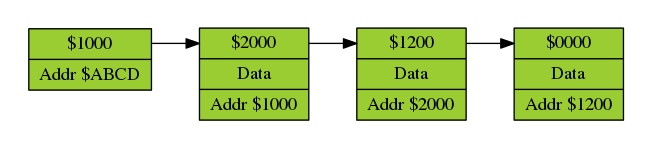
\includegraphics[width=0.95\textwidth]{Content/images/LL_Single_Memory.png}
\caption{Memory Organisation of a Simple Linked List.}
\label{fig:MemoryOrganisationOfASimpleLinkedList}
\end{figure}

You can see from \figurename~\ref{fig:MemoryOrganisationOfASimpleLinkedList} that the address of the following node is held in each node's first 4
    bytes. The address of FIRST is actually somewhere in your program
    and your program only needs to allocate storage for the 4 bytes it takes
    to hold the address of the initial node in the list. FIRST is, of course,
    the root node of the list.

You must store the value zero in there before you go off adding
    nodes, you'll see this reason why below in the code to add a node.

\subsection{Adding Nodes.}
\label{ch10-adding-nodes}%\hyperlabel{ch10-adding-nodes}%

Adding a new node is simple, you allocate it on the heap, fill in
      the data part and add it to the front of the list. It is far easier to
      add a node at the start -{} address 1000 in the above example -{} than to
      have to work through the entire list to find the current end, and then
      add it there. This method takes longer and longer to carry out as you
      add extra entries to the list. Adding at the start of the list takes the
      same time regardless of how many entries are in the list.

As you add each node to the list, you copy the value in FIRST into
      the new node's NEXT pointer and put the address of the new node into
      FIRST. Sounds complicated, but here it is in code. If we assume that
      A0.L has the address of FIRST and that A1.L has the address of the node
      to be inserted into the list, as contrivingly demonstrated by these two
      lines:

\begin{lstlisting}[firstnumber=1,caption={Adding a Node - Prelude},label={lst:AddingANodePrelude}]
Prelude    lea FIRST,a0        ; Pointer to storage of first node 
           lea NewEntry,a1     ; Address of new node
\end{lstlisting}

Then adding a new node to a list is as simple as this:

\begin{lstlisting}[firstnumber=last,caption={Adding a Node},label={lst:AddingANode}]
AddNode    move.l (a0),(a1)    ; Save first node in new node's NEXT
           move.l  a1,(a0)     ; Store new node in FIRST
           rts
\end{lstlisting}

Nothing to it. The new node is always added at the start of the
      list, so the value in FIRST always points to the most recently added
      node. As you need to have zero in the NEXT pointer of the final node in
      the list, you can see why it was important to initialise the value in
      your programs FIRST variable to zero before adding any nodes. If you
      didn't have zero, you'd never know when the list was finished.

One thing, you don't want to allow the user to add the root node
      to its own list at any time, so best change the above code to prevent
      this from happening.

\begin{lstlisting}[firstnumber=3,caption={A Better Way of Adding a Node},label={lst:BetterAddingANode}]
AddNode    cmpa.l  a0,a1       ; Don't allow the root node to be added
           beq.s   AddExit     ; Bale out quietly if attempted
           move.l (a0),(a1)    ; Save first node in new node's NEXT
           move.l  a1,(a0)     ; Store new node in FIRST
AddExit    rts
\end{lstlisting}

Another problem is when you try to add a node that is already
      there. So to be really careful, you could call the FindNode routine
      (coming soon -{} have patience!) prior to adding it in. However, as this
      scans the entire list until it finds or doesn't find the new node, it
      could add quite a lot of time to the simple exercise of adding a new
      node.

If you wrote the program, and you are allocating nodes on the heap
      each time, then don't bother attempting to find the node in the list
      before you add it.

\subsection{Deleting Nodes.}
\label{ch10-deleting-nodes}%\hyperlabel{ch10-deleting-nodes}%

Deleting a node is slightly more difficult. The node to be deleted
      could be anywhere in the list, or not even in the list. How to find the
      correct node is the main problem. However, for the same of argument,
      assume that we have the node address to be removed in A1.L and the
      address of FIRST in A0.L after a successful `find' operation, then
      removing the node at A1.L requires that we must navigate the list, as in
      the following explanation.

We must navigate the list because we don't know where in memory
      the node prior to the one we wish to delete is. We need to find it,
      because it has a NEXT pointer holding the address of the `deleted' node
      and this has to be changed or we lose everything in the list after the
      deleted node.

As ever, the value in the NEXT area of the very last node in the
      list is always zero. That way, we know when we have hit the end of the
      list. Here's the pseudo code to delete the node at A1.L from the list
      beginning at (A0.L)
\begin{itemize}[itemsep=0pt]

\item{}If the node to be deleted is the root node (the list pointer
          in A0) then don't allow it to be deleted.


\item{}Start of the main loop.


\item{}If the value stored in the address that A0.L points to is
          equal to zero, we have been passed an incorect node address to
          delete. Exit from the loop with an error.


\item{}If the value stored in the address that A0.L points to is not
          the same as the value in A1.L then copy the value in the address
          that A0.L points to into A0 and restart the main loop. Basically we
          have replaced the address in A0 with the NEXT address from the node
          we were just looking at.


\item{}If the value stored in the address that A0.L points to is
          equal to the value in A1.L then we have found the node PRIOR to the
          node we wish to delete and so the node we are looking at has to have
          the NEXT address updated to bypass the node we wish to delete so
          that it now points to the NEXT address which is currently stored in
          the node we are deleting. Exit from the loop with no errors.


\item{}End of main loop.

\end{itemize}

That's the pseudo code, here's the actual code. Using the same
      preliminary stuff as above to sort out initial values of A0.L and A1.L
      and a little bit extra to show whether errors have been detected or not,
      we begin with this:

\begin{lstlisting}[firstnumber=1,caption={Deleting a Node - Prelude},label={lst:DeletingANodePrelude}]
Prelude    lea FIRST,a0        ; Pointer to root node
           lea OldNode,a1      ; Address of node to delete
           moveq #ERR_EF,d0    ; End of file = node not found = error
\end{lstlisting}

Now, here's the actual code to find and remove the requested
      node.

\begin{lstlisting}[firstnumber=last,caption={Deleting a Node},label={lst:DeletingANode}]
DelNode    cmpa.l a0,a1        ; Don't allow the root node deletion
           beq.s DelExit       ; Bale out with error if attempted

DelLoop    cmp.l #0,(a0)       ; Reached the end yet?
           beq.s DelExit       ; Yes, node not found, exit with error

           cmp.l (a0),a1       ; Found the PRIOR node yet?
           bne.s DelNext       ; No, skip deletion code & try again

DelFound   move.l (a1),(a0)    ; PRIOR node NEXT = deleted node's NEXT 
           moveq  #0,d0        ; Node found and deleted ok
           bra.s  DelExit      ; Bale out with no errors

DelNext    move.l (a0),a0      ; A0 now holds the NEXT node in the list
           bra.s  DelLoop      ; Go around again

DelExit    tst.l d0            ; Set zero flag for success
           rts
\end{lstlisting}

The above code returns with the Z flag set if the node was deleted
      from the list, and unset if the node was not in the list. This allows
      the calling code to handle and errors correctly.

\subsection{Finding Nodes.}
\label{ch10-finding-nodes}%\hyperlabel{ch10-finding-nodes}%

The first thing you must do when deleting a node is to actually
      find it. The code above assumes that A1 holds a valid node address in
      the list defined by A0. Having said that, the code is robust enough to
      know that programmers make errors and it can handle the problem of a
      node address being passed which is not in the list by virtue of the fact
      that it scans the list until it finds the node prior to the one we wish
      to delete. It has to work that way because we need to adjust the NEXT
      pointer in the prior node to point past the deleted node to its NEXT
      node -{} if you catch my drift?

The code to find an node in a list is dependant on the sort of
      data stored in each node. If you store strings, the some form of string
      comparison routine needs to be built in -{} does it compare on an equality
      basis (`AAA' = `AAA') or nearly equal basis (`AAA' == `aaa') and so on.
      You can use the built in QDOSMSQ routines to do the comparisons.

If the data in the nodes are numbers (integers of word or long
      length) then you can compare them directly. If they are QDOSMSQ floating
      point format numbers, you can use the built in arithmetic routines to
      compare them. Regardless of which method is used, you need to write your
      own code to compare two nodes, or a node and a value so that the find
      routine knows when it has found the correct entry.

Of course, it is quite simple to build a FindNode routine which
      doesn't know or care what sort of data the individual nodes contain,
      provided it is passed the address of a routine which does know and care.
      If the specification for said routine requires the Z flag to be set for
      found and unset for not found, it could look something like the
      following peseudo code.

Assume that A0.L holds the address of FIRST, A1.L holds a pointer
      to a routine which compares the node with a given value and A2.L holds a
      pointer to that value. The data that A2.L points to can be anything, the
      routine at (A1.L) does the working out, our FindNode simply calls the
      routine once for each node in the list until such time as it gets a set
      Z flag on return. The comparison routine gets passed a node address in
      A3.L.
\begin{itemize}[itemsep=0pt]

\item{}Start of the main loop.


\item{}If the value stored in the address that A0.L points to is
          equal to zero, we have not found a node with the desired value. Exit
          the main loop with a NOT FOUND error.


\item{}Copy the address at (A0.L) into A3 and call the routine to
          compare data. If it returns with the Z flag set, the address in
          (A0.L) is the address of the node prior to the node we were looking
          for, however, the address in A3.L is the address of our required
          node as it is taken from the NEXT pointer. Remember, we passed the
          NEXT address (A0.L) over to the routine, not the address of THIS
          node -{} A0.L. Exit from the loop with the Z flag set to indicate a
          found node.


\item{}Copy the NEXT address from the node we are looking at into
          A0.L and go back to the start of the loop.


\item{}End of main loop.

\end{itemize}

And here's the real code to do the finding for use. As ever, we
      start off with some contrived values.

\begin{lstlisting}[firstnumber=1,caption={Finding a Node - Prelude},label={lst:FindingANodePrelude}]
Prelude    lea FIRST,a0        ; Pointer to root node address
           lea Compare,a1      ; Address of node comparison routine
           lea Required,a2     ; Address of the data we are looking for
           moveq #ERR_NF,d0    ; Node not found = error
\end{lstlisting}

Now, here's the actual code to find a node in the list which holds
      the required value.

\begin{lstlisting}[firstnumber=last,caption={Finding a Node},label={lst:FindingANode}]
FindNode   cmp.l #0,(a0)       ; Reached the end yet?
           beq.s DelExit       ; Yes, node not found, exit with error

           move.l (a0),a3      ; Fetch the NEXT node address into A3.L
           jsr (a1)            ; And jump into the comparison routine
           beq.s FindFound     ; Looks like we found our node

FindNext   move.l (a0),a0      ; A0 now holds the NEXT node in the list
           bra.s  FindNode     ; Go around again

FindFound  moveq  #0,d0        ; Clear the error flag

FindExit   tst.l d0            ; Set zero flag for success
           rts
\end{lstlisting}

The following is an example of a compare routine to look at a long
      word of data in the node at (A3.L) and see if it is equal to the long
      word of data stored at (A2.L). Don't forget, the comparison routine must
      preserve A0, A1, A2 and D0 or it will all go horribly wrong. The
      following routine does exactly that, by the simple method of not
      actually using those registers at all!

\begin{lstlisting}[firstnumber=1,caption={Finding a Node - Data Comparison},label={lst:FindingANodeDataComparison}]
NData   equ 4                  ; Offset to node's data part

Compare    cmp.l NData(A3),(A2) ; Is the data = the value we want?
           rts                 ; Exit with Z set if so
\end{lstlisting}

If an attempt is made to find the root node, then it will
      fail.

So there you have three short but extremely powerful routines
      which make linked lists possible. At this point I have to mention that
      there are actually routines built into QDOSMSQ to do exactly the same
      work as the AddNode and DelNode routines above, but there is nothing
      like FindNode -{} which is a shame. However, you now know how to build
      linked lists and add and delete nodes. You also know how to find an
      entry in a linked list so that you can process it in some way.

\subsection{The Code Wrapper.}\index{Linked Lists!Test Harness}
\label{ch10-code-wrapper}%\hyperlabel{ch10-code-wrapper}%

Putting all of the above together and tying in some extras to
      allocate nodes etc, here is a small, but perfectly formed program to
      create a linked list. The following is a wrapper that we shall use to
      demonstrate first the single linked lists as explained above. Later on,
      when other types of linked list are explained, we shall drop in only the
      code we need for the demo

\begin{lstlisting}[firstnumber=1,caption={Linked Lists - Wrapper - Part 1},label={LinkedListsWrapperPart1}]
* =====================================================================
* A test harness 'job' for our linked lists code. What's the point of
* all the explanations if you can't test the code?
*
* This code is simply a wrapper to allow different demos to be slotted
* in to demonstrate the real code in the chapter, as opposed to the job
* code.
*
* The code being demonstrated is located at DEMO below. As new demos
* are required, only that bit should (!) need changing.
* =====================================================================

* ---------------------------------------------------------------------
* These are offsets from the start of the job's dataspace where working
* variable are stored. The dataspace is held at (A4) in the job's code.
* ---------------------------------------------------------------------
con_id      equ     0                   ; Id for title channel
con_id2     equ     4                   ; Id for main output

* ---------------------------------------------------------------------
* These are simply user friendly names instead of numbers for various
* bits and bobs, colours etc.
* ---------------------------------------------------------------------
black       equ     0                   ; Colour code for mode 4 black
red         equ     2                   ; Red
green       equ     4                   ; Green
white       equ     7                   ; White
linefeed    equ    10                   ; Linefeed character
oops        equ    -1                   ; General error code
err_nc      equ    -1                   ; NOT COMPLETE error code

* ---------------------------------------------------------------------
* Constants for use with job control commands. (It doesn't matter if I
* have two names with the same value! )
* ---------------------------------------------------------------------
infinite    equ     -1                  ; Infinite timeout
me          equ     -1                  ; Id for 'this' job


* ---------------------------------------------------------------------
* Code starts here.
* ---------------------------------------------------------------------
start       bra.s   LinkList            ; 2 bytes short jump
            dc.l    0                   ; 4 bytes padding
            dc.w    $4afb
            dc.w    11                  ; Bytes in job's name
            dc.b    'LinkedLists',0     ; Bytes of job's name + padding

LinkList    adda.l   a6,a4              ; A4.L = start of dataspace
            bsr      Mode4              ; Set the screen mode
            bsr      Title              ; Open the title window
            bsr      Output             ; Open the output window
            bsr      Headings           ; Display headings
            bsr      Demo               ; Do the demo code
            bsr      Finished           ; Advise user that we are done

* ---------------------------------------------------------------------
* Code ends here.
* ---------------------------------------------------------------------
all_done    moveq   #mt_frjob,d0        ; Force Remove a job
            moveq   #me,d1              ; The current job
            move.l  d0,d3               ; Error code for SuperBasic
            trap    #1                  ; Kill this job

            bra.s   all_done            ; Should never get here
\end{lstlisting}

\begin{note}
The following code will be replaced by either the singly linked
        list or the doubly linked list demo code which follows at the end of
        this chapter. For now, however, it is a place holder.
\end{note}

\begin{lstlisting}[firstnumber=last,caption={Linked Lists - Wrapper - Demo Placeholder},label={LinkedListsWrapperDemoPlaceholder}]
* ---------------------------------------------------------------------
* The DEMO code starts here.
* ---------------------------------------------------------------------
Demo        rts

* ---------------------------------------------------------------------
* The DEMO code ends here.
* ---------------------------------------------------------------------
\end{lstlisting}

\begin{note}
The following code is common to both demos.
\end{note}

\begin{lstlisting}[firstnumber=last,caption={Linked Lists - Wrapper - Part 2},label={LinkedListsWrapperPart2}]
* ---------------------------------------------------------------------
* Set mode 4 if not already set. Do not change from TV to monitor or
* vice versa. We must preserve the display type if we reset the mode.
* ---------------------------------------------------------------------
Mode4       moveq    #mt_dmode,d0
            moveq    #-1,d1             ; Read current mode
            moveq    #-1,d2             ; Read current display type
            trap     #1                 ; Do it
            tst.l    d0                 ; Did it work?
            bne      all_done           ; No, bale out, cannot continue

            tst.b    d1                 ; 0 in D1.B = Mode 4
            beq.s    ModeExit           ; No need to set mode 4
            moveq    #mt_dmode,d0
            clr.l    d1                 ; We need mode 4
            trap     #1                 ; Set mode 4 (d2 = disp type)
            tst.l    d0                 ; Check it
            bne      all_done           ; Bale out if errors detected
ModeExit    rts                         ; Done.

* ---------------------------------------------------------------------
* Mode 4 is in use. Open the title window at the top of the screen.
* ---------------------------------------------------------------------
Title       lea      con_def,a1         ; Window definition
            movea.w  ut_con,a2          ; Utility to define a window
            jsr      (a2)               ; Do it
            tst.l    d0                 ; Did it work ok?
            bne      all_done           ; No, exit program
            move.l   a0,con_id(a4)      ; Store title channel id
            rts                         ; Done

*----------------------------------------------------------------------
* Definition for title window channel
*----------------------------------------------------------------------
con_def     dc.b    red                 ; Border colour
            dc.b    1                   ; Border width
            dc.b    white               ; Paper/strip colour
            dc.b    black               ; Ink colour
            dc.w    448                 ; Width
            dc.w    24                  ; Height
            dc.w    32                  ; Start position x
            dc.w    16                  ; Start position y

* ---------------------------------------------------------------------
* Open the output window underneath the title one.
* ---------------------------------------------------------------------
Output      lea      con_def2,a1        ; Output window definition
            movea.w  ut_con,a2          ; Utility again
            jsr      (a2)               ; Do it
            tst.l    d0                 ; Did it work?
            bne      all_done           ; No, exit routine
            move.l   a0,con_id2(a4)     ; Store output channel id

            moveq    #0,d0              ; No errors detected
            rts

*----------------------------------------------------------------------
* Definition for output window channel
*----------------------------------------------------------------------
con_def2    dc.b    red                 ; Border colour
            dc.b    1                   ; Border width
            dc.b    white               ; Paper/strip colour
            dc.b    black               ; Ink colour
            dc.w    448                 ; Width
            dc.w    200                 ; Height
            dc.w    32                  ; X org
            dc.w    40                  ; Y org

* ---------------------------------------------------------------------
* Print the headings
* ---------------------------------------------------------------------
headings    movea.l  con_id(a4),a0       ; Title channel id
            bsr.s    cls                 ; Clear screen
            lea      mes_title,a1        ; Title string
            bsr.s    prompt              ; Print title string
            rts

mes_title   dc.w     mes_end-mes_title-2
            dc.b     'Single Linked Lists'
mes_end     equ      *

* ---------------------------------------------------------------------
* Sign off message
* ---------------------------------------------------------------------
Finished    movea.l  con_id2(a4),a0      ; Title channel id
            lea      end_title,a1        ; Title string
            bsr.s    prompt              ; Print title string
            bsr.s    input               ; Wait for ENTER
            rts

end_title   dc.w     end_end-end_title-2
            dc.b     linefeed,linefeed,'Press ENTER to quit: '
end_end     equ      *

* =====================================================================
* CLS:
* =====================================================================
* 1. Clear the (screen) channel whose id is in A0.
* =====================================================================
cls         moveq    #sd_clear,d0        ; CLS
            moveq    #infinite,d3        ; Infinite timeout
            trap     #3                  ; CLS title window
            rts

* =====================================================================
* Prompt:
* =====================================================================
* 1. Print the string at (A1) to the channel in A0.
*
* Z set if all ok, unset if not.
* =====================================================================
prompt      movea.w ut_mtext,a2          ; Print a string utility
            jsr     (a2)                 ; Print it
            tst.l   d0                   ; Check for errors
            rts

* =====================================================================
* Input:
* =====================================================================
* Wait for user input from the channel id in A0.
*
* Returns the input length (not counting the ENTER character) in D1.W
* Returns the address of the first character in the buffer in A1.L
* Preserves the channel id in A0.L
* Z set if all ok, unset if not.
* =====================================================================
input       lea     buffer+2,a1         ; Our buffer address plus 2
            move.l  a1,-(a7)            ; Save it on the stack
            moveq   #io_fline,d0        ; Input some bytes (+ linefeed)
            moveq   #60,d2              ; Buffer size maximum
            moveq   #infinite,d3        ; Inifinite timeout
            trap    #3

            move.l  (a7)+,a1            ; Restore buffer pointer
            subq.w  #1,d1               ; Subtract the linefeed
            move.w  d1,-2(a1)           ; Store length in buffer
            tst.l   d0                  ; Did it all work?
            rts

buffer      ds.w    31                  ; 60 chars for input + 1 word

* =====================================================================
* hex_l:
* =====================================================================
* Convert a 4 byte value in D4.L to Hex in a buffer. Use the input
* buffer for the output and DOES NOT store the length word!
*
* Expects D4.L to hold the value.
* =====================================================================
hex_l       swap    d4              ; $ABCD -> $CDAB in D4
            bsr.s   hex_w           ; Convert the $AB part first
            swap    d4              ; $CDAB -> $ABCD again
*           drop into hex_w to convert the $CD part

* =====================================================================
* hex_w:
* =====================================================================
* Convert a 2 byte value in D4.W to Hex in a buffer.
*
* Expects D4.W to hold the value.
* Expects A1.L to point at the buffer.
* =====================================================================
hex_w       ror.w   #8,d4           ; $DE -> $ED in D4
            bsr.s   hex_b           ; Convert the $D part first
            rol.w   #8,d4           ; $ED -> $DE again
*           drop into hex_b to convert the $E part

* =====================================================================
* hex_b:
* =====================================================================
* Convert a 1 byte value in D4.B to Hex in a buffer.
*
* Expects D4.B to hold the value.
* Expects A1.L to point at the buffer.
* =====================================================================
hex_b       ror.b   #4,d4           ; Swap lower and higer nibbles
            bsr.s   hex_nibble      ; Print high nibble first
            rol.b   #4,d4           ; Swap back again
*           drop into hex_nibble to print the lower nibble

* =====================================================================
* hex_nibble:
* =====================================================================
* Convert a 4 bit value in D4.B to Hex in a buffer.
*
* Expects D4.B to hold the value.
* Expects A1.L to point at the buffer.
* =====================================================================
hex_nibble  move.b  d4,-(a7)        ; Save value in both nibbles
            andi.b  #$0f,d4         ; D4.B now = 0 to 15
            addi.b  #'0',d4         ; Now = '0' to '?' (ascii only)
            cmpi.b  #'9',d4         ; Is this a digit?
            bls.s   nib_digit       ; Yes
            addi.b  #7,d4           ; Add offset to UPPERCASE letters

nib_digit   move.b  d4,(a1)+        ; Store in buffer
            move.b  (a7)+,d4        ; Restore original value
            rts

* =====================================================================
* print_hex:
* =====================================================================
* Convert D4 into 8 hex characters, and print it to the channel in A0.L
*
* Expects D4.L to hold the value.
* Expects A0.L to hold the channel id.
* =====================================================================
print_hex   lea      buffer,a1      ; Output buffer for address
            move.w   #8,(a1)+       ; We know the result is 8 bytes
            bsr      hex_l          ; Convert 4 bytes to text
            lea      buffer,a1      ; Text to print
            bsr      prompt         ; Print it
            rts                     ; All done. (Error code in D0)

* =====================================================================
* End of test harness
* =====================================================================
\end{lstlisting}

\subsection{Running The Wrapper Code.}
\label{ch10-single-list}%\hyperlabel{ch10-single-list}%

The above code does absolutely nothing, but if you assemble it and
      exec the resulting file, you should see a pair of windows one with a
      message `Single Linked Lists' and a prompt in the other to `Press ENTER
      to quit'. Once you press the ENTER key, the job will finish. So far so
      good.

The reason that it does nothing is shown below:

\begin{lstlisting}[firstnumber=1,caption={Linked Lists - Wrapper - Demo Placeholder},label={LinkedListsWrapperDemoPlaceholder2}]
* =====================================================================
* The DEMO code starts here.
* =====================================================================
Demo        rts

* =====================================================================
* The DEMO code ends here.
* =====================================================================
\end{lstlisting}

The code at Demo, does nothing but return to the caller. Our
      linked list code will be slotted in to replace the lines of code shown
      above.

To demonstrate linked lists, we need only add some code to replace
      the lines above. In the following two chapters we do just that, and code
      to demonstrate single and doubly linked lists follows there. 

\subsection{Problem Areas.}
\label{ch10-problems}%\hyperlabel{ch10-problems}%

The above description, and code, is for a Single Linked List, so
      called because there is a single link in each node which points to the
      next entry in the list. This is simple to code up -{} as we have seen -{}
      and is fairly simple to understand, at least it is if I've done my job
      correctly.

The problem with a linked list created in the above fashion is
      that you always have to scan the list from start to some undetermined
      entry when you want to delete a node. And this can add serious delays to
      the processing of your application when a lot of nodes have to be
      traversed each time you need to delete one.

There is an answer, Doubly Linked Lists.

\section{Doubly Linked Lists.}
\label{ch10-double-lists}%\hyperlabel{ch10-double-lists}%

If we change the structure of our nodes and add a PRIOR pointer to
    each node and to the root node as well, we can store the address of both
    nodes neighbouring our current one, as shown in  Figure~\ref{fig:StructureOfADoubleLinkedListNode} which shows the node structure.
    
\begin{note}
Simon N Goodwin pointed out some time ago that there is no need to have two separate pointers for prior and next nodes in the linked list, only one pointer is needed.

This pointer holds the address of both pointers \opcode{EOR}'d together. To extract the prior pointer, simply \opcode{EOR} it with the next address and vice versa.

This assumes that you know the address of the prior and/or next pointer I suspect!
\end{note}    

\begin{figure}[h]
\center
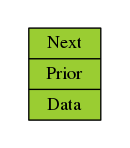
\includegraphics[width=0.2\textwidth]{Content/images/LL_Double_node.png}
\caption{Structure of a Doubly Linked List Node.}
\label{fig:StructureOfADoubleLinkedListNode}
\end{figure}

Our conceptual model of the doubly linked list is shown in Figure~\ref{fig:ConceptualModelOfADoublyLinkedList}.

\begin{figure}[h]
\center
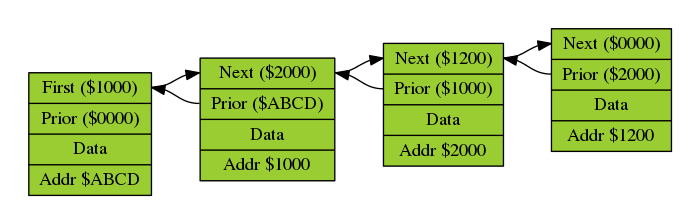
\includegraphics[width=0.95\textwidth]{Content/images/LL_Double_list.png}
\caption{Conceptual Model of a Doubly Linked List.}
\label{fig:ConceptualModelOfADoublyLinkedList}
\end{figure}

\subsection{Adding Nodes.}
\label{ch10-dbl-adding-nodes}%\hyperlabel{ch10-dbl-adding-nodes}%

Adding a new node is still simple. Having allocated a node on the
      heap, you set its PRIOR pointer to zero and its NEXT to the current
      address held in the FIRST pointer -{} almost identical to the single
      linked list code above.

\begin{lstlisting}[firstnumber=1,caption={Adding a Node - Prelude},label={lst:AddingANodePrelude2}]
Prior      equ 4               ; Offset to PRIOR pointer in a node

Prelude    lea FIRST,a0        ; Pointer to root node
           lea NewEntry,a1     ; Address of new node
\end{lstlisting}

Then adding a new node to a doubly linked list is as simple as
      this:

\begin{lstlisting}[firstnumber=last,caption={Adding a Node},label={lst:AddingANode2}]
AddNode    cmpa.l  a0,a1         ; Don't add the root node again
           beq.s   AddExit       ; Bale out quietly if attempted
           move.l (a0),(a1)      ; Save first node in new node's NEXT 
           move.l  a0,Prior(a1)  ; Set the PRIOR node for this new node
           move.l  a1,(a0)       ; Store new node in FIRST 
           move.l  (a1),a0       ; A0 = address of original FIRST node
           cmpa.l  #0,a0         ; Nothing to do if A0 is zero
           beq.s   AddExit       ; Z set = First node added
           move.l  a1,prior(a0)  ; Store new FIRST node
AddExit    rts
\end{lstlisting}

As with single linked lists there is nothing to it. The new node
      is always added at the start of the list, so the value in FIRST always
      points to the latest node added. The first non root node in a doubly
      linked list has no real PRIOR node, so that part of the newly added node
      is simply set to point back at the root node.

Building up the linked list above, in Figure~\ref{fig:ConceptualModelOfADoublyLinkedList}, in stages, we would start with the root node located, most likely, somewhere in our code itself. Initially both the next and prior pointers would be set to zero.

The nodes are address at the start of the list, so the first node to be added would be the one on the far right of the diagram, node \$1200. That node would be created and added to the list by setting the root node's next pointer to address \$1200 and the new node's prior pointer to address \$ABCD. Because it is the final node in the list so far, its next pointer is set to zero.

After adding the node at address \$2000, we would change the next pointer of the root node to this new address, \$2000, and the prior pointer of the node at \$1200 to \$2000. The new node would have its prior pointer set to the address that was in the \$1200 node's prior pointer, which is \$ABCD.

This process is repeated as we create each new node and add it to the list. Eventually, we end up with the structure shown in Figure~\ref{fig:ConceptualModelOfADoublyLinkedList} above.

You can see how each node points onward to the NEXT one and also
      backwards to the PRIOR one. The last node has no NEXT nodes, so it has
      its NEXT pointers set to zero to indicate the end of the list.

\subsection{Deleting Nodes.}
\label{ch10-dbl-deleteing-nodes}%\hyperlabel{ch10-dbl-deleteing-nodes}%

Deleting a node is much simpler. There is no need to scan the
      entire list from the start looking for the node prior to the one you
      want to delete because you already know its address by following the
      PRIOR pointer backwards from the node to be deleted.

Here's the pseudo code to delete a node. We assume, as before,
      that A0.L is the root node pointer and A1.L is the node to be
      deleted.
\begin{itemize}[itemsep=0pt]

\item{}If the two addresses are equal, we cannot allow the root node
          to be deleted, exit with an error.


\item{}If the address in the root node's NEXT pointer is zero then we
          still have an empty list so the value in A1 must be illegal. Exit
          with an error.


\item{}Fetch the deleted node's PRIOR pointer. Every real node in a
          list will have a valid PRIOR pointer, only the root node has no
          prior pointer and we don't allow that to be deleted.


\item{}Store the NEXT pointer from the deleted node into the NEXT
          pointer of the prior node.


\item{}Fetch the deleted node's NEXT pointer, which might be zero if
          we are deleting the final node in the list.


\item{}If it is not zero, store the deleted node's PRIOR pointer in
          the next node's PRIOR pointer.


\item{}Exit without error.

\end{itemize}

That's the pseudo code, here's the real code to do all of the
      above.

\begin{lstlisting}[firstnumber=1,caption={Deleting a Node - Prelude},label={lst:DeletingANodePrelude2}]
Prior      equ 4               ; Offset to PRIOR pointer in each node

Prelude    lea FIRST,a0        ; Pointer to root node
           lea OldNode,a1      ; Address of node to delete
           moveq #ERR_BP,d0    ; Trying to delete the root node?
\end{lstlisting}

Now, here's the actual code to find and remove the requested
      node.

\begin{lstlisting}[firstnumber=last,caption={Deleting a Node},label={lst:DeletingANode2}]
DelNode    cmpa.l a0,a1        ; Don't delete the root node
           beq.s DelExit       ; Bale out with error if attempted

           cmp.l #0,(a0)       ; Do we actually have a list?
           beq.s DelExit       ; Yes, node not found, exit with error

           move.l Prior(a1),a0 ; Fetch the deleted node's PRIOR pointer
           move.l (a1),(a0)    ; Store its NEXT pointer in the NEXT
                               ; pointer of the PRIOR node

           move.l (a1),a0      ; Fetch the deleted node's NEXT pointer
           move.l  Prior(a1),Prior(a0) ; Store its PRIOR pointer in the
                                       ; next node's PRIOR pointer.

DelFound   move.l (a1),(a0)    ; PRIOR's NEXT = the deleted node's NEXT
           moveq  #0,d0        ; Node deleted ok
           bra.s  DelExit      ; Bale out with no errors

DelNext    move.l (a0),a0      ; A0 now holds the NEXT node in the list
           bra.s  DelNode      ; Go around again

DelExit    tst.l d0            ; Set zero flag for success
           rts
\end{lstlisting}

\subsection{Finding Nodes.}
\label{ch10-dbl-finding-nodes}%\hyperlabel{ch10-dbl-finding-nodes}%

As with single linked lists, you may have a need to locate a
      specific node by its contents, so you need a generic FindNode routine
      again. The fact that the list has two pointers this time around is the
      only difference, so the code is basically the same as for the single
      linked list above.

The only difference is the offset to the data part of the node
      needs to be set to 8 bytes instead of 4, so while the code for the
      FindNode remains the same, the code for the Compare routine needs to be
      changed to the following to account for the extra pointer.

As before, the comparison routine must preserve A0, A1, A2 and D0
      or it will all go horribly wrong.

\begin{lstlisting}[firstnumber=1,caption={Finding a Node - Data Comparison},label={lst:FindingANodedataComparison2}]
NData   equ 8                  ; Offset from start of node to the data

Compare    cmp.l NData(a3),(a2) ; Is the data = the value we want?
           rts                  ; Exit with Z set if so
\end{lstlisting}

Again, if an attempt is made to `find' the root node, then it will
      fail.

\subsection{A Better Mousetrap.}
\label{ch10-better-mousetrap}%\hyperlabel{ch10-better-mousetrap}%

Because the code for the linked list find routine is identical
      except for the offset in the compare routine you can use the same code.
      If you modify it so that it passes the offset over to the compare
      routine in a spare register, say D1.W for example, then you can even
      have the same compare routine for both single and doubly linked lists,
      as shown below.

\begin{lstlisting}[firstnumber=1,caption={Finding a Node - Data Comparison},label={lst:FindingANodedataComparison3}]
Compare    cmp.l 0(a3,d1.w),(a2) ; Is the data = the value we want?
           rts                   ; Exit with Z set if so
\end{lstlisting}

Another method, much loved in the internals of Microsoft Windows,
      is to store a word holding the offset to the data at the start of each
      node. This would remove the need for the D1.W register to be passed into
      the comparison routine as a parameter as it could easily extract the
      data from the node itself, as follows:

\begin{lstlisting}[firstnumber=1,caption={Finding a Node - Alternative Data Comparison},label={lst:FindingANodedataComparison4}]
Compare    move.w (a3),d1        ; Fetch the offset to the data
           cmp.l 0(a3,d1.w),(a2) ; Is the data = the value we want?
           rts                   ; Exit with Z set if so
\end{lstlisting}

The drawback to this method is the redundancy of the data -{} each
      and every node has to have the first two bytes set to the offset to the
      data plus 2 for the size of the offset word itself. Two extra bytes per
      node may be the difference between getting all the data in memory or
      not. It is, of course, always up to you. If you decide to go down this
      route, don't forget to amend the code to add, find and delete nodes to
      take the extra two bytes into consideration when manipulating the
      pointers to NEXT and PRIOR. Your root node must also reflect these
      changes and have an offset word added to its own structure.

You might see a need to build a couple of comparison routines to
      compare two nodes rather than the example above where a node is being
      compared with a value. On the other hand, you could simply write one
      routine to compare two nodes and when looking for a value, create a
      dummy node and use that in the comparison routine. That way, you don't
      need separate routines to compare values and nodes.

\subsection{Double Trouble.}
\label{ch10-double-trouble}%\hyperlabel{ch10-double-trouble}%

The problem with a doubly linked list is that while adding nodes
      is just as simple as before, but deleting them could be problematical.
      If you are passed the address of a node which is not in the list, how do
      you tell that it is or is not a valid node address? You can end up
      trashing bytes of memory almost at random as you start changing the NEXT
      and PRIOR pointers for two areas of memory which may not be in your
      list.

My solution is to use a flag word or long word after the two list
      pointers in each node and when passed in a node address to delete,
      compare this value in the flag to see if it is correct before attempting
      to delete the node. As ever, I leave this `as an exercise for the
      reader' to modify the code above to carry out said checks.

\subsection{Sorting Lists.}
\label{ch10-sorting-lists}%\hyperlabel{ch10-sorting-lists}%

The best way to sort a list is not to have to sort it at all. When
      you store a node in the list, store it in the correct place according to
      its value. A doubly linked list is used here again as you will need to
      go NEXT until you hit a value greater than the one you want to insert,
      then you might need to go PRIOR to insert it in the correct location.
      I'll leave you to figure out that little exercise.

There is an another way, which involves TREES of nodes rather than
      lists. A tree is simply a linked list which has a LEFT, RIGHT and UP
      pointer in each node.

With a tree, the nodes are not in a long line, but they are off to
      the LEFT and RIGHT of the root node. Each node may itself have children
      to the LEFT and RIGHT as well as a parent found by following the UP
      pointer.

Unfortunately, trees are a bit beyond my skills at the moment. I
      remember doing them in college and learning all the different ways to
      navigate them, but I cannot remember much about them nowadays -{} it's
      been over 30 years since I last considered them.

\section{Remember those arrays?}
\label{ch10-remember-arrays}%\hyperlabel{ch10-remember-arrays}%

Way back at the start of this chapter, I mentioned arrays and their
    problems. Well, combining an array with a linked list could be useful -{}
    but remember, the array is limited by the fact that you have to pre-{}define
    the number of entries.

Bearing this in mind, you could allocate an array of, say 1000
    entries of 4 bytes each. Each entry in the array holds the address of an
    individual node, not the actual data stored there. Our address book system
    of 100 byte strings (not much of an address book I admit!) will now only
    need about 4Kb plus 102 bytes per used node -{} including the string length
    word for each entry. Using a plain array it would need almost 102Kb even
    for a blank address book.

Now you have compromised on memory needs as you don't allocate the
    space required to store your data until you need to, and you do allocate a
    much smaller amount to hold the `contents table'. As you create new nodes,
    add their address to the array. You can still use the single or double
    linked lists if you wish, but there is no need. The array holds all the
    locations of each node in the order that they were created and you can
    navigate forwards, backwards and even access nodes at random using this
    method because the formula to find a given node is once more
    usable.

Have fun trying that out!

\section{Coming Up...}
\label{ch10-the-end}%\hyperlabel{ch10-the-end}%

Coming up next, the real code for the single linked list demo, and
    following that, the code for the doubly linked list demo.

